\documentclass[10pt,a4paper,danish]{article}
%% Indlæs ofte brugte pakker
\usepackage{amssymb}
\usepackage[danish]{babel}
\usepackage[utf8]{inputenc}
\usepackage{listings}
\usepackage{fancyhdr}
\usepackage{hyperref}
\usepackage{booktabs}
\usepackage{graphicx}
\usepackage{todonotes}
\usepackage{algorithmic}
\usepackage{amsmath}


\pagestyle{fancy}
\fancyhead{}
\fancyfoot{}
\rhead{\today}
\rfoot{\thepage}
\setlength{\parindent}{0pt}

% Opsæt indlæsning af filer
\lstset{
 language=Python,
 extendedchars=\true,
 inputencoding=utf8,
 linewidth=\textwidth, basicstyle=\small,
 numbers=left, numberstyle=\footnotesize,
 tabsize=2, showstringspaces=false,
 breaklines=true, breakatwhitespace=false,
}

%% Titel og forfatter
\title{G1\\Maskinarkitektur\\Efterår 2011}
\author{Jens Fredskov\\ Naja Mottelson (vsj465)\\Søren Pilgård (vpb984)}

%% Start dokumentet
\begin{document}

%% Vis titel
\maketitle
\newpage

%% Vis indholdsfortegnelse
\tableofcontents
\newpage

%% Klar, parat, start!
\section{Indledning}
Nærværende rapport tjener som dokumentation af gruppens arbejde med første
godkendelsesopgave. Den indeholder korrekte og afprøvede løsninger på samtlige
underopgaver. 

\section{g1-1}
På Figur \ref{fig:circ1} ses vores implementation af de grundlæggende logiske
gates (AND, OR, NOT, XOR) vha. NAND-gates. Som det ses følger vores implementering
metoden i lærebogens Appendix C. 

\begin{figure}[htb]
\begin{center}
\leavevmode
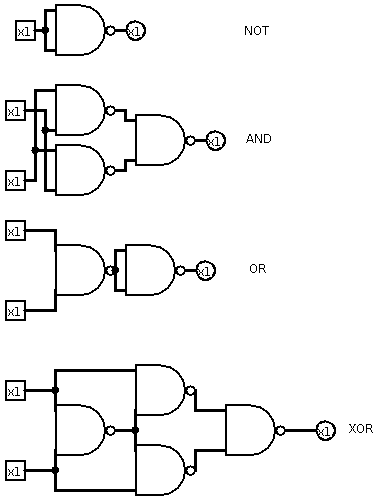
\includegraphics[scale=0.70]{circ1.png}
\end{center}
\caption{NOT-, AND-, OR- og XOR-gates af NAND-gates}
\label{fig:circ1} 
\end{figure}

\section{g1-2} 
Overordnet er vores 4-bit ALU (se Figur \ref{fig:circ2}) implementeret som en serie af fire 1-bit ALU'er
(se Figur \ref{fig:alu-1bit}) efter samme logik som den 32-bit ALU der præsenteres i Appenix C-29. Her 
forbindes CarryOut-outputtet fra de mindre betydende bits til CarryIn-inputtet for de mere betydende. 
Nedenfor er en gennemgang af de operationer 1-bit ALU'en understøtter og deres implementering: 

\begin{description}
\item[AND, OR] ALU'ens grundlæggende logiske funktioner benytter de indbyggede gates i logisim.
\item[NOR] Outputtet til NOR udregnes som NOT A AND NOT B. Til dette benyttes multiplekserne 
           Ainvert og Binvert. 
\item[Addér] ALU'en benytter et Adder-modul (se Figur \ref{fig:adder-1bit}), som vi i gruppen har 
             implementeret vha. logisims Combinatorial Analysis-værktøj og sandhedstabellen i Figur C.53. 
\item[Subtrahér] Substraktionsfunktionen benytter samme Adder, blot med én af operanderne inverteret. 
\item[Set Less Than] Set Less Than-operationen (SLT) er en komposit operation: Først sammenlignes A og B, 
                     hvilket giver resultatet 1 hvis A $<$ B, 0 ellers. Herefter sættes alle inputtets bits
                     til 0, med undtagelse af den mindst betydende bit som sættes til resultatet af 
                     sammenligningen. I forbindelse med 1-bit ALU'en giver SLT derfor ikke så megen mening
                     (NB! Er dette overhovedet korrekt? Logikken virker da udmærket, hvis man tager Set
                     som output. Men det er vel defineret således at Result er det eneste output vi 
                     interesserer os for?)
\item[ZERO] Zero-outputtet er separat fra Result-outputtet og beregned ved at føre output-signalet fra 
            de andre operationer igennem en XNOR-gate. (NB! Er Zero overhovedet defineret for 1-bit ALU'en?)
\end{description}

Som det ses adskiller seriens sidste 1-bit ALU (som håndterer den mest betydende bit i inputtet) sig fra de
foregående ved at understøtte yderligere funktionalitet til håndtering af SLT-operationen samt at undersøge
for overløb. Udover overløbsmodulet (se Figur \ref{fig:overflow}) har vi implementeret denne del af logikken
efter samme algoritme som beskrives i Appendix C-31-C-35. 

\begin{figure}[htb]
\begin{center}
\leavevmode
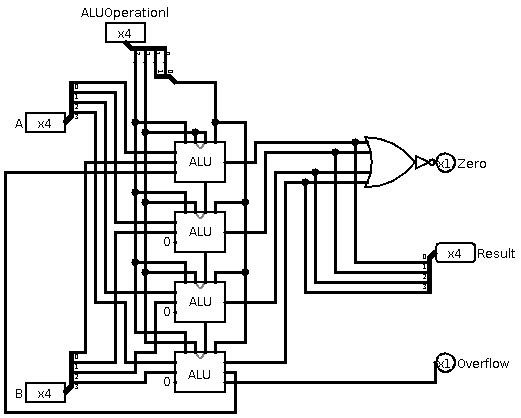
\includegraphics[scale=0.70]{circ2.png}
\end{center}
\caption{ALU, 4-bit}
\label{fig:circ2}
\end{figure}

\begin{figure}[htb]
\begin{center}
\leavevmode
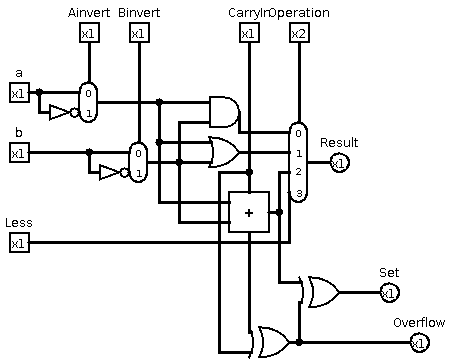
\includegraphics[scale=0.70]{alu-1bit-overflow.png}
\end{center}
\caption{1-bit ALU m. undersøgelse af overløb}
\label{fig:alu-1bit}
\end{figure}

\subsection{Multiplexer}

\begin{figure}[htb]
\begin{center}
\leavevmode
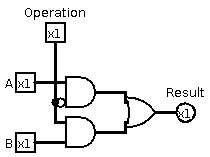
\includegraphics[scale=0.70]{mux-2bit.png}
\end{center}
\caption{MUX, 2 bit IN}
\label{fig:mux2bit} 
\end{figure}

\begin{figure}[htb]
\begin{center}
\leavevmode
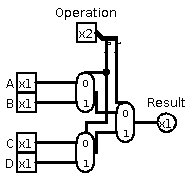
\includegraphics[scale=0.70]{mux-4bit.png}
\end{center}
\caption{MUX, 4 bit IN}
\label{fig:mux4bit} 
\end{figure}

\subsection{Adder}
\begin{figure}[htb]
\begin{center}
\leavevmode
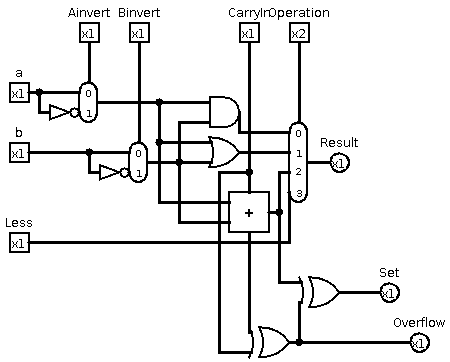
\includegraphics[scale=0.70]{adder-1bit.png}
\end{center}
\caption{1-bit adder}
\label{fig:adder}
\end{figure}

\subsection{Overløbskontrol}
\begin{figure}[htb]
\begin{center}
\leavevmode
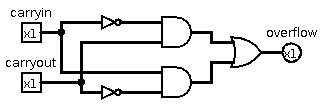
\includegraphics[scale=0.70]{overflow-detection.png}
\end{center}
\caption{Logikken til undersøgelse af overløb}
\label{fig:overflow}
\end{figure}

\section{g1-3}


\paragraph{}
NB! Mangler argumentation for korrekthed/afprøvning!




\end{document}
